% Construction : une courbe continue de (a, f(a)) à (b, f(b)) avec a = 0,6 et
% b = 5,2 ; la valeur intermédiaire k = 1,9 est atteinte en c = 2,9.
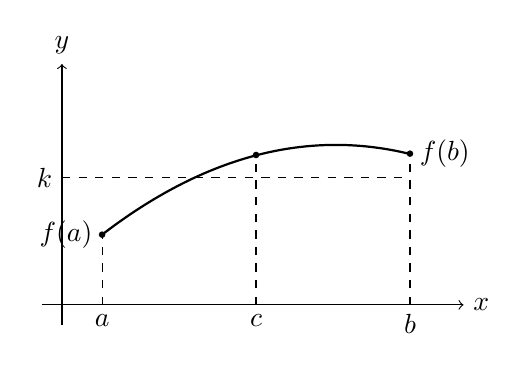
\begin{tikzpicture}[scale=0.85]
  \draw[->] (-0.3, 0) -- (6, 0) node[right] {$x$};
  \draw[->] (0, -0.3) -- (0, 3.6) node[above] {$y$};
  \draw[thick, domain=0.6:5.2, smooth, variable=\x]
    plot ({\x}, {0.55 + 0.9*\x - 0.11*\x*\x});
  \draw[dashed] (0, 1.9) node[left] {$k$} -- (5.2, 1.9);
  \draw[dashed] (0.6, 0) node[below] {$a$} -- (0.6, 1.05);
  \draw[dashed] (5.2, 0) node[below] {$b$} -- (5.2, 2.26);
  \draw[dashed] (2.9, 0) node[below] {$c$} -- (2.9, 2.24);
  \fill (0.6, 1.05) circle (1.4pt) node[left] {$f(a)$};
  \fill (5.2, 2.26) circle (1.4pt) node[right] {$f(b)$};
  \fill (2.9, 2.24) circle (1.4pt);
\end{tikzpicture}
